\chapter{Positive Definite Matrices}

A fundamental class of symmetric matrices behaves in many respects like
\emph{positive numbers}. They have positive eigenvalues and positive pivots, their
determinants are positive, and they admit unique positive definite square roots. They define quadratic
forms that are strictly positive for every nonzero vector, providing the foundation for convex
optimization, covariance analysis in statistics (which records how pairs of variables fluctuate
together), Hessians at local minima in multivariable calculus (matrices of second derivatives that
certify upward curvature), stiffness matrices in structural mechanics (measuring how firmly a
structure resists deformation), and positive definite kernels in machine learning (functions that
measure similarity between data points). These are the \emph{positive definite} matrices.

If the spectral theorem of the previous chapter told you that every symmetric matrix is a set of
perpendicular axes with a stretch factor on each, then this chapter asks the next natural question:
\emph{what if every stretch factor is positive?} The answer turns out to reorganize a huge amount of
linear algebra around a single, very physical idea: \textbf{energy}.

\section{The energy of a matrix}

\subsection{From a number to a matrix}

Start with the humblest object: a single positive number $a > 0$. What does ``positive'' buy you?
Multiplying by $a$ never flips a sign: $a x$ has the same sign as $x$. The function $f(x) = a x^2$
is a bowl opening upward with its bottom at $x = 0$; it is positive for every $x \neq 0$. You can
take a square root $\sqrt{a}$. Every one of these facts has a matrix analogue, and the matrices that
inherit them are exactly the positive definite ones.

Here is the bridge. For a number $a$, the quantity $a x^2 = x \, a \, x$ is the ``energy.'' For an
$n \times n$ symmetric matrix $\mat{A}$ and a vector $\vec{x} \in \R^n$, the analogue is the scalar

\[
  q(\vec{x}) \;=\; \vec{x}\T \mat{A}\, \vec{x}.
\]

This single number -- a vector, times a matrix, times the same vector again -- runs through the
whole chapter. It is called a \textbf{quadratic form}: a multivariable polynomial where every single
term has degree two (such as $2x_1^2 + 2x_1 x_2 + 3x_2^2$), with no linear or constant pieces. Here
is what it actually computes.

\begin{example}[Unpacking $\vec{x}\T\mat{A}\vec{x}$ by hand]
\label{ch27:ex-unpack}
Take
\[
  \mat{A} = \begin{bmatrix} 2 & 1 \\ 1 & 3 \end{bmatrix}, \qquad
  \vec{x} = \colvec{x_1 \\ x_2}.
\]
Compute $\mat{A}\vec{x}$ first:
\[
  \mat{A}\vec{x} = \colvec{2x_1 + x_2 \\ x_1 + 3x_2}.
\]
Now dot it with $\vec{x}$:
\[
  \vec{x}\T \mat{A}\vec{x}
  = x_1(2x_1 + x_2) + x_2(x_1 + 3x_2)
  = 2x_1^2 + 2x_1 x_2 + 3x_2^2.
\]
The diagonal entries $2$ and $3$ became the coefficients of $x_1^2$ and
$x_2^2$. The off-diagonal entry $1$ appears \emph{twice} (once as $A_{12}$, once as $A_{21}$), and
those two copies combine into the single cross term $2 x_1 x_2$. A symmetric matrix is exactly a
bookkeeping device for a quadratic in several variables.
\end{example}

In general, expanding the product gives the clean formula

\[
  \vec{x}\T \mat{A}\, \vec{x} \;=\; \sum_{i=1}^n \sum_{j=1}^n A_{ij}\, x_i x_j
  \;=\; \sum_i A_{ii}\, x_i^2 \;+\; 2\sum_{i<j} A_{ij}\, x_i x_j,
\]

where the last step used $A_{ij} = A_{ji}$. The diagonal carries the pure squares; the
off-diagonal carries the interactions.

\begin{intuitionbox}
Think of $\vec{x}\T\mat{A}\vec{x}$ as the \emph{height of a curved surface} above the input point $\vec{x}$.
For an ordinary number $a>0$, $f(x) = ax^2$ is a parabola -- a 1D valley. For a matrix, $q(\vec{x})$
is a multidimensional surface. The entire question of this chapter is: \emph{is that surface a bowl
that curves up in every direction?} If yes, $\mat{A}$ is positive definite.
\end{intuitionbox}

\begin{trapbox}
Only the \emph{symmetric part} of a matrix affects the quadratic form. If $\mat{A}$ is not
symmetric, then $\vec{x}\T\mat{A}\vec{x} = \vec{x}\T \mat{A}_{\text{sym}}\,\vec{x}$ where
$\mat{A}_{\text{sym}} = \tfrac12(\mat{A} + \mat{A}\T)$, because the antisymmetric part contributes
nothing: $\vec{x}\T \mat{B}\vec{x} = 0$ whenever $\mat{B}\T = -\mat{B}$. So when we talk about
positive definiteness we \emph{always} assume $\mat{A}$ is symmetric -- otherwise we just replace it
by its symmetric part and lose nothing.
\end{trapbox}

\subsection{The definition}

\begin{definition}[Positive definite]
\label{ch27:def-pd}
A symmetric matrix $\mat{A} \in \R^{n\times n}$ is \textbf{positive definite} (PD) if
\[
  \vec{x}\T \mat{A}\, \vec{x} \;>\; 0 \qquad \text{for every nonzero } \vec{x} \in \R^n.
\]
It is \textbf{positive semidefinite} (PSD) if the weaker $\vec{x}\T\mat{A}\vec{x} \geq 0$ holds for
all $\vec{x}$. We write $\mat{A} \succ 0$ for positive definite and $\mat{A} \succeq 0$ for positive
semidefinite. Reversing the inequalities gives \emph{negative (semi)definite}; a matrix whose form
takes both positive and negative values is \textbf{indefinite} (meaning the surface bends up along
some directions and down along others, forming a saddle).
\end{definition}

\begin{recoverybox}
\textbf{Mental check.} Why does Definition~\ref{ch27:def-pd} demand $\vec{x}\T\mat{A}\vec{x} > 0$
for \emph{nonzero} $\vec{x}$, rather than all $\vec{x}$? Because at $\vec{x} = \vec{0}$, the form
$\vec{0}\T\mat{A}\vec{0}$ is identically zero for every matrix. The heart of positive definiteness
is that as soon as you step away from the origin in \emph{any} direction, the energy strictly climbs.
\end{recoverybox}

The requirement ``for every nonzero $\vec{x}$'' is essential. At $\vec{x} = \vec{0}$ the form is
always $0$, so we exclude it; the demand is that \emph{moving away from the origin in any direction
whatsoever} strictly increases the value. That is precisely what makes a bowl a bowl.

\begin{focusbox}
Hold onto this one sentence: \emph{positive definite means the quadratic surface
$\vec{x}\T\mat{A}\vec{x}$ is a bowl that opens strictly upward in every direction, with its unique
lowest point at the origin.} Everything else in this chapter -- eigenvalue tests, pivot tests,
determinant tests, Cholesky, covariance -- is a different way of certifying that one geometric fact.
\end{focusbox}

\subsection{Three quadratic surfaces}

A $2\times 2$ quadratic form can be one of three qualitatively different things. Plotting
$z = \vec{x}\T\mat{A}\vec{x}$ over the plane shows the difference instantly.

\begin{figure}[H]
\centering
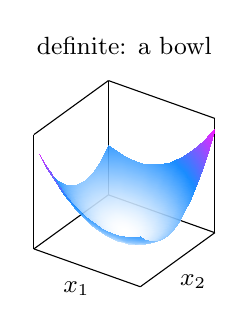
\begin{tikzpicture}
\begin{axis}[
  width=0.32\textwidth, height=4.2cm, view={35}{30},
  xlabel={\small$x_1$}, ylabel={\small$x_2$},
  ticks=none, title={definite: a bowl}, title style={font=\small},
  domain=-1.2:1.2, y domain=-1.2:1.2, samples=20, colormap/cool, z buffer=sort]
  \addplot3[surf, shader=interp, opacity=0.9] {2*x^2 + 2*x*y + 3*y^2};
\end{axis}
\end{tikzpicture}\hfill
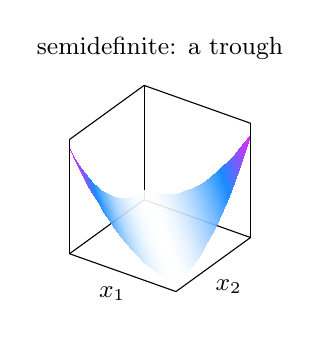
\begin{tikzpicture}
\begin{axis}[
  width=0.32\textwidth, height=4.2cm, view={35}{30},
  xlabel={\small$x_1$}, ylabel={\small$x_2$},
  ticks=none, title={semidefinite: a trough}, title style={font=\small},
  domain=-1.2:1.2, y domain=-1.2:1.2, samples=20, colormap/cool, z buffer=sort]
  \addplot3[surf, shader=interp, opacity=0.9] {(x+y)^2};
\end{axis}
\end{tikzpicture}\hfill
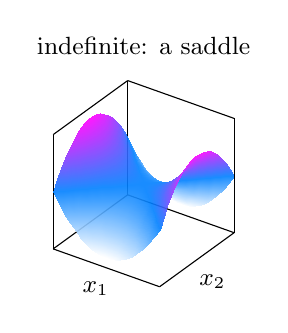
\begin{tikzpicture}
\begin{axis}[
  width=0.32\textwidth, height=4.2cm, view={35}{30},
  xlabel={\small$x_1$}, ylabel={\small$x_2$},
  ticks=none, title={indefinite: a saddle}, title style={font=\small},
  domain=-1.2:1.2, y domain=-1.2:1.2, samples=20, colormap/cool, z buffer=sort]
  \addplot3[surf, shader=interp, opacity=0.9] {x^2 - y^2};
\end{axis}
\end{tikzpicture}
\caption{The three faces of a quadratic form $z=\vec{x}\T\mat{A}\vec{x}$. \emph{Left:} positive
definite -- every cross-section through the origin curves up, so the only minimum is at the bottom.
\emph{Middle:} positive semidefinite -- a flat-bottomed trough; it never dips below zero but stays at
zero along a whole line. \emph{Right:} indefinite -- the form rises in one direction and falls in
another, a saddle with no minimum.}
\label{ch27:fig-three-surfaces}
\end{figure}

The left surface is $2x_1^2 + 2x_1x_2 + 3x_2^2$ from the positive definite $\mat{A}$ of
Example~\ref{ch27:ex-unpack}. The middle is
$(x_1+x_2)^2$, which is never negative but \emph{equals zero} along the entire line $x_1 = -x_2$ --
that is the signature of semidefinite: a direction of zero energy. The right is $x_1^2 - x_2^2$, a
saddle: walk along $x_1$ and the form climbs, walk along $x_2$ and it drops. Recognizing which
picture you are in is what the tests below let you do without ever drawing the surface.

\section{Test 1: eigenvalues}

The cleanest characterization comes straight from the spectral theorem. Because $\mat{A}$ is
symmetric, it has real eigenvalues $\lambda_1, \dots, \lambda_n$ and an \emph{orthonormal} basis of
eigenvectors $\vec{q}_1, \dots, \vec{q}_n$:
\[
  \mat{A} = \mat{Q}\,\mat{\Lambda}\,\mat{Q}\T, \qquad
  \mat{Q}\T\mat{Q} = \mat{I}, \quad \mat{\Lambda} = \diag(\lambda_1,\dots,\lambda_n).
\]
Now substitute this into the energy and change coordinates. Let $\vec{y} = \mat{Q}\T\vec{x}$ (the
coordinates of $\vec{x}$ in the eigenvector basis). Then
\[
  \vec{x}\T\mat{A}\vec{x}
  = \vec{x}\T\mat{Q}\mat{\Lambda}\mat{Q}\T\vec{x}
  = (\mat{Q}\T\vec{x})\T \mat{\Lambda}\, (\mat{Q}\T\vec{x})
  = \vec{y}\T\mat{\Lambda}\vec{y}
  = \lambda_1 y_1^2 + \lambda_2 y_2^2 + \cdots + \lambda_n y_n^2.
\]

This is the most important computation in the chapter. \emph{In the eigenvector
coordinates the cross terms vanish.} The messy form $\sum A_{ij} x_i x_j$ becomes a clean weighted
sum of pure squares, and the weights are the eigenvalues. Because $\mat{Q}$ is an orthogonal matrix,
$\vec{x} = \vec{0}$ if and only if $\vec{y} = \vec{0}$, so asking ``is the form positive for all
$\vec{x}\neq\vec{0}$?'' becomes ``is $\sum \lambda_i y_i^2 > 0$ for all $\vec{y}\neq\vec{0}$?'' --
and that holds exactly when every $\lambda_i > 0$.

\begin{theorem}[Eigenvalue test]
\label{ch27:thm-eig}
A symmetric matrix $\mat{A}$ is positive definite if and only if all of its eigenvalues are
strictly positive. It is positive semidefinite iff all eigenvalues are $\geq 0$.
\end{theorem}

\begin{proof}
($\Leftarrow$) If every $\lambda_i > 0$ and $\vec{x}\neq\vec{0}$, then $\vec{y}=\mat{Q}\T\vec{x}
\neq\vec{0}$, so at least one $y_k \neq 0$, and $\sum \lambda_i y_i^2 \geq \lambda_k y_k^2 > 0$.
($\Rightarrow$) Conversely, suppose $\mat{A}\succ 0$ and let $\vec{q}_k$ be a unit eigenvector for
$\lambda_k$. Plug $\vec{x} = \vec{q}_k$ into the form:
$\vec{q}_k\T\mat{A}\vec{q}_k = \vec{q}_k\T(\lambda_k\vec{q}_k) = \lambda_k \norm{\vec{q}_k}^2 =
\lambda_k$. Positive definiteness forces this to be $>0$, so $\lambda_k > 0$. The semidefinite
statement is identical with $\geq$.
\end{proof}

\begin{example}[Reading positivity off the eigenvalues]
\label{ch27:ex-eig}
For $\mat{A} = \begin{bmatrix} 2 & 1 \\ 1 & 3 \end{bmatrix}$ the characteristic equation is
\[
  \det(\mat{A} - \lambda\mat{I}) = (2-\lambda)(3-\lambda) - 1 = \lambda^2 - 5\lambda + 5 = 0,
  \qquad \lambda = \frac{5 \pm \sqrt 5}{2}.
\]
That gives $\lambda_1 \approx 3.618$ and $\lambda_2 \approx 1.382$, both positive, so $\mat{A}\succ
0$. Two sanity checks you can do in your head: the trace $\lambda_1 + \lambda_2 = 5 = 2+3$ matches
the diagonal sum, and the product $\lambda_1\lambda_2 = 5 = \det\mat{A}$. Both being positive is
\emph{consistent} with PD, though as we will see the determinant alone is not enough.
\end{example}

\begin{trapbox}
A positive determinant does \emph{not} guarantee positive definiteness. Consider
$\begin{bmatrix} -2 & 0 \\ 0 & -3 \end{bmatrix}$: its determinant is $+6 > 0$, but both eigenvalues
are negative, so the form $-2x_1^2 - 3x_2^2$ is negative everywhere. A positive determinant in 2D
only says the eigenvalues have the \emph{same} sign -- they could both be negative. You need more,
which is why the determinant test below inspects \emph{all} the leading principal minors, rather than the
final determinant alone.
\end{trapbox}

\section{Test 2: pivots}

Computing eigenvalues means solving a polynomial -- exact but expensive. There is a much cheaper
test hiding inside elimination, the very first algorithm you ever learned. Recall that Gaussian
elimination without row swaps factors a matrix as $\mat{A} = \mat{L}\mat{U}$, where $\mat{L}$ is
lower triangular with ones on the diagonal and $\mat{U}$ is upper triangular. The diagonal entries
of $\mat{U}$ are the \textbf{pivots} (the non-zero leading values used to clear the column entries
below them during elimination).

\begin{theorem}[Pivot test]
\label{ch27:thm-pivots}
A symmetric matrix $\mat{A}$ is positive definite if and only if elimination runs to completion
\emph{without any row exchanges} and produces $n$ \emph{strictly positive pivots}.
\end{theorem}

\begin{recoverybox}
\textbf{Mental check.} Suppose you begin elimination on a symmetric matrix $\mat{A}$ and find
$A_{11} \leq 0$. Can $\mat{A}$ possibly be positive definite? No -- because $A_{11}$ is the very first
pivot $d_1$, and it also equals the energy of the first standard basis vector:
$\vec{e}_1\T\mat{A}\vec{e}_1 = A_{11}$. If $A_{11} \leq 0$, the test vector $\vec{e}_1 = (1, 0, \dots, 0)\T$
already gives zero or negative energy, so the matrix fails positive definiteness before elimination takes
a single step.
\end{recoverybox}

Here is why this is believable, and where it comes from. For a symmetric $\mat{A}$ the
$\mat{L}\mat{U}$ factorization can be made symmetric: $\mat{A} = \mat{L}\,\mat{D}\,\mat{L}\T$, where
$\mat{D} = \diag(d_1,\dots,d_n)$ holds the pivots. (This is the symmetric cousin of $\mat{LU}$;
$\mat{U} = \mat{D}\mat{L}\T$.) Substitute into the energy and set $\vec{y} = \mat{L}\T\vec{x}$:
\[
  \vec{x}\T\mat{A}\vec{x}
  = \vec{x}\T\mat{L}\mat{D}\mat{L}\T\vec{x}
  = (\mat{L}\T\vec{x})\T \mat{D} (\mat{L}\T\vec{x})
  = \vec{y}\T\mat{D}\vec{y}
  = d_1 y_1^2 + d_2 y_2^2 + \cdots + d_n y_n^2.
\]
Because $\mat{L}\T$ is invertible (ones on the diagonal), $\vec{x}\neq\vec{0}$ iff
$\vec{y}\neq\vec{0}$. So exactly as with eigenvalues, the form is a weighted sum of squares -- only
now the weights are the \emph{pivots}, not the eigenvalues. Positivity of the form is equivalent to
positivity of every pivot. (The pivots and eigenvalues are generally different numbers; both sets
happen to be all-positive together. Only the \emph{determinant} is shared by the two sets,
$\det\mat{A} = \prod d_i = \prod \lambda_i$; the trace equals the sum of eigenvalues but \emph{not}
the sum of pivots -- for $\begin{bmatrix}2&1\\1&3\end{bmatrix}$ the pivots $2,\tfrac52$ sum to
$\tfrac92$, while the trace is $5$.)

\begin{example}[Completing the square is elimination]
\label{ch27:ex-square}
Take $\mat{A} = \begin{bmatrix} 2 & 1 \\ 1 & 3 \end{bmatrix}$ again. One elimination step subtracts
$\tfrac12$ times row 1 from row 2:
\[
  \mat{A} \;\longrightarrow\;
  \mat{U} = \begin{bmatrix} 2 & 1 \\ 0 & \tfrac52 \end{bmatrix},
  \qquad \text{pivots } d_1 = 2,\; d_2 = \tfrac52.
\]
Both positive, so $\mat{A}\succ 0$. And watch the pivots reappear when you \emph{complete the
square} on the quadratic form directly:
\[
  2x_1^2 + 2x_1 x_2 + 3x_2^2
  = \underbrace{2}_{d_1}\Big(x_1 + \tfrac12 x_2\Big)^2 + \underbrace{\tfrac52}_{d_2}\, x_2^2 .
\]
The pivot $2$ multiplies the completed square; the pivot $\tfrac52$ multiplies the leftover. The
multiplier $\tfrac12$ inside the parenthesis is exactly the $L_{21}$ entry from elimination. Two
positive coefficients in front of two squares $\Rightarrow$ the form is a sum of nonnegative pieces
that vanish only at $\vec{x}=\vec{0}$. \emph{Completing the square and Gaussian elimination are the
same computation.}
\end{example}

\begin{strangbox}
Strang loves to say ``the pivots tell you the signs.'' This is the place that pays off. In his
course the $\mat{LDL}\T$ factorization and the energy test appear together, and the punch line is
exactly Example~\ref{ch27:ex-square}: each pivot is the coefficient of a completed square. If you
read this chapter \emph{before} Strang, the thing to carry in is that elimination does far more than solve
$\mat{A}\vec{x}=\vec{b}$ -- it is also an immediate positivity detector. If you are here \emph{after}
Strang, notice that the pivot test is what makes positive definiteness \emph{cheap}: $O(n^3)$
elimination versus solving for eigenvalues.
\end{strangbox}

\section{Test 3: leading minors (the determinant test)}

There is a third test, beautiful because it requires no factorization at all -- just determinants of
the top-left corners. The $k$th \textbf{leading principal minor} $\Delta_k$ is the determinant of the
top-left $k\times k$ block of $\mat{A}$ (the square submatrix formed by the first $k$ rows and columns).

\begin{theorem}[Sylvester's criterion]
\label{ch27:thm-sylvester}
A symmetric matrix $\mat{A}$ is positive definite if and only if every leading principal minor is
positive:
\[
  \Delta_1 = A_{11} > 0,\quad
  \Delta_2 = \det\begin{bmatrix} A_{11} & A_{12} \\ A_{21} & A_{22}\end{bmatrix} > 0,\quad
  \dots,\quad
  \Delta_n = \det\mat{A} > 0.
\]
\end{theorem}

The link to the pivot test makes this almost obvious. The $k$th pivot equals a ratio of consecutive
leading minors,
\[
  d_k = \frac{\Delta_k}{\Delta_{k-1}}, \qquad (\Delta_0 := 1),
\]
because the product of the first $k$ pivots is the determinant of the top-left $k\times k$ block.
If all $\Delta_k > 0$ then every ratio $d_k = \Delta_k/\Delta_{k-1} > 0$, so all pivots are
positive and $\mat{A}\succ 0$ by Theorem~\ref{ch27:thm-pivots}; conversely positive pivots make
every $\Delta_k = d_1 d_2\cdots d_k > 0$.

\begin{example}[All three tests on one matrix]
\label{ch27:ex-allthree}
Let
\[
  \mat{A} = \begin{bmatrix} 2 & -1 & 0 \\ -1 & 2 & -1 \\ 0 & -1 & 2 \end{bmatrix},
\]
the famous ``second difference'' matrix. Run every test.

\emph{Leading minors:} $\Delta_1 = 2 > 0$; $\Delta_2 = \det\begin{bmatrix}2&-1\\-1&2\end{bmatrix}
= 3 > 0$; $\Delta_3 = \det\mat{A} = 2(4-1) - (-1)(-2-0) = 6 - 2 = 4 > 0$. All positive: PD.

\emph{Pivots:} elimination gives $d_1 = \Delta_1 = 2$, $d_2 = \Delta_2/\Delta_1 = 3/2$, $d_3 =
\Delta_3/\Delta_2 = 4/3$. All positive, and their product confirms $2 \cdot \tfrac32 \cdot \tfrac43 = 4 = \det\mat{A}$.

\emph{Eigenvalues:} for this matrix they are known in closed form, $\lambda_k = 2 - 2\cos\frac{k\pi}{4}$
for $k=1,2,3$, giving $2-\sqrt2 \approx 0.586$, $2$, and $2+\sqrt2 \approx 3.414$ -- all positive.
Three tests, three different sets of positive numbers, one verdict: $\mat{A}\succ 0$.
\end{example}

\begin{labbox}
Test $\mat{B} = \begin{bmatrix} 1 & 2 \\ 2 & 1 \end{bmatrix}$ by all three methods and confirm they
agree that it is \emph{not} positive definite.
\emph{Minors:} $\Delta_1 = 1 > 0$ but $\Delta_2 = 1 - 4 = -3 < 0$. The failure of $\Delta_2$ is the
red flag.
\emph{Pivots:} $d_1 = 1$, then eliminate to get $d_2 = -3$. A negative pivot.
\emph{Eigenvalues:} $\lambda = 1 \pm 2$, i.e. $3$ and $-1$. The negative eigenvalue means the form
$x_1^2 + 4x_1x_2 + x_2^2$ is a saddle -- try $\vec{x}=(1,-1)$ to get $1 - 4 + 1 = -2 < 0$.
\end{labbox}

\begin{trapbox}
Sylvester's criterion uses the \emph{leading} (top-left) minors and is a test for \emph{positive
definiteness only}. Do not try to detect positive \emph{semi}definiteness by relaxing to
$\Delta_k \geq 0$ -- that is false. The matrix $\begin{bmatrix} 0 & 0 \\ 0 & -1\end{bmatrix}$ has
$\Delta_1 = 0$ and $\Delta_2 = 0$, both $\geq 0$, yet it is negative semidefinite, not positive. For
semidefiniteness you must check \emph{all} principal minors (every diagonal sub-block, rather than only the
leading ones), or simply fall back to the eigenvalue test $\lambda_i \geq 0$.
\end{trapbox}

\section{The geometry: ellipses and ellipsoids}

We have three algebraic tests. The geometry behind them is what makes positive definiteness feel
inevitable, and the right picture is not the 3D bowl but its \emph{level sets} -- the curves where the
energy is constant.

For a positive definite $2\times2$ matrix, the set
\[
  \{\,\vec{x} : \vec{x}\T\mat{A}\vec{x} = 1\,\}
\]
is an \textbf{ellipse} centered at the origin. (If $\mat{A}$ were indefinite you would get a
hyperbola; if singular semidefinite, a pair of parallel lines.) The ellipse is the constant-energy
contour, and positive definiteness is exactly the statement that these contours are \emph{closed
loops} hugging the origin rather than open curves running off to infinity.

The spectral decomposition tells you the ellipse's shape precisely. In the eigenvector coordinates
$\vec{y} = \mat{Q}\T\vec{x}$, the equation $\vec{x}\T\mat{A}\vec{x}=1$ becomes
\[
  \lambda_1 y_1^2 + \lambda_2 y_2^2 = 1,
\]
the standard equation of an ellipse with semi-axis lengths $1/\sqrt{\lambda_1}$ and
$1/\sqrt{\lambda_2}$ along the eigenvector directions $\vec{q}_1, \vec{q}_2$.

\begin{focusbox}
\textbf{The eigenvectors are the axes of the ellipse; the eigenvalues set the axis lengths.} A
\emph{large} eigenvalue means the form grows fast in that direction, so the contour is \emph{close}
to the origin there (short axis $1/\sqrt\lambda$). A \emph{small} eigenvalue means a long, shallow axis.
Positive definite $\Leftrightarrow$ both axes are real and finite $\Leftrightarrow$ the contour is a
genuine ellipse.
\end{focusbox}

\begin{figure}[H]
\centering
\begin{tikzpicture}[scale=1.55,>=Stealth]
  % axes
  \draw[->,spacegray] (-1.6,0) -- (1.8,0) node[right]{\footnotesize$x_1$};
  \draw[->,spacegray] (0,-1.6) -- (0,1.8) node[above]{\footnotesize$x_2$};

  % concentric ellipses for A = [[2,1],[1,2]] rotated 45 deg:
  % semi-axes: sqrt(c)/sqrt(3) and sqrt(c)/sqrt(1)
  \begin{scope}[rotate=45]
    % c = 0.5: 0.408 and 0.707
    \fill[vecblue!6] (0,0) ellipse (0.408 and 0.707);
    \draw[vecblue!50, dashed] (0,0) ellipse (0.408 and 0.707);
    % c = 1.0: 0.577 and 1.000
    \draw[vecblue, very thick] (0,0) ellipse (0.577 and 1.000);
    % c = 1.6: 0.730 and 1.265
    \draw[vecblue!70, thick] (0,0) ellipse (0.730 and 1.265);
  \end{scope}

  % eigen-axes lines
  \draw[vecred!35, dashed] (-1.2,-1.2) -- (1.4,1.4);
  \draw[targetgreen!35, dashed] (-1.3,1.3) -- (1.3,-1.3);

  % eigenvectors
  \draw[->,vecred,very thick] (0,0) -- (0.408,0.408) node[below right=1pt,font=\scriptsize] {$\vec q_1\,(\lambda_1=3)$};
  \draw[->,targetgreen,very thick] (0,0) -- (0.707,-0.707) node[below right=2pt,font=\footnotesize,fill=white,inner sep=1.5pt] {$\vec q_2\,(\lambda_2=1)$};

  % contour labels
  \node[font=\tiny, fill=white, inner sep=1.5pt, rounded corners=1pt, text=vecblue!80!black] at (0.28,0.62) {$c=0.5$};
  \node[font=\tiny, fill=white, inner sep=1.5pt, rounded corners=1pt, text=vecblue!90!black] at (0.55,0.92) {$c=1.0$};
  \node[font=\tiny, fill=white, inner sep=1.5pt, rounded corners=1pt, text=vecblue!90!black] at (0.82,1.20) {$c=1.6$};

  % annotations
  \node[font=\footnotesize, targetgreen!80!black] at (1.1,-1.35) {long axis $=1/\sqrt{\lambda_2}=1$};
  \node[font=\footnotesize, vecred!80!black] at (-0.9,-1.1) {short axis $=1/\sqrt{\lambda_1}$};
\end{tikzpicture}
\caption{Concentric energy contours $\vec{x}\T\mat{A}\vec{x}=c$ of the positive definite
quadratic form $\mat{A}=\begin{bmatrix}2&1\\1&2\end{bmatrix}$. The eigenvectors
$\vec{q}_1,\vec{q}_2$ point along the principal axes. The largest eigenvalue ($\lambda_1=3$)
steepens the bowl and compresses the level curve into the \emph{short} axis ($1/\sqrt3$);
the smaller eigenvalue ($\lambda_2=1$) yields the \emph{long} axis ($1$). Positive
definiteness ensures every contour is a closed, nested ellipse.}
\label{ch27:fig-ellipse}
\end{figure}

In $\R^n$ the same statement holds: the level set $\vec{x}\T\mat{A}\vec{x} = 1$ is an
\textbf{ellipsoid} with principal axes along the eigenvectors and semi-axis lengths
$1/\sqrt{\lambda_i}$. In this sense, a positive definite matrix corresponds directly to a geometric ellipsoid. This
geometric interpretation is central whenever covariance matrices or Hessians appear: the level sets of
the associated quadratic forms are concentric ellipsoids.

\begin{walkbox}
Consider the contour $\vec{x}\T\mat{A}\vec{x}=1$ as one eigenvalue decreases toward $0$.
The semi-axis $1/\sqrt\lambda$ in that direction stretches toward infinity, and the ellipse elongates into an
unbounded cylinder. When $\lambda = 0$, the matrix is positive semidefinite and the
level set is unbounded. If $\lambda$ becomes negative, the surface becomes a hyperboloid (or hyperbola in two dimensions), reflecting indefiniteness. Thus, strictly positive eigenvalues correspond precisely to closed, bounded ellipsoidal contours.
\end{walkbox}

\section{Cholesky: the square root of a matrix}

A positive number $a>0$ has a square root $\sqrt a$, and you can write $a = (\sqrt a)(\sqrt a)$.
Positive definite matrices inherit this too, and the matrix version is one of the most useful
factorizations in all of computation.

\begin{theorem}[Cholesky factorization]
\label{ch27:thm-cholesky}
A symmetric matrix $\mat{A}$ is positive definite if and only if it can be written
\[
  \mat{A} = \mat{R}\T\mat{R}
\]
for some upper-triangular matrix $\mat{R}$ with \emph{strictly positive} diagonal entries. This
$\mat{R}$ is unique, and is called the \textbf{Cholesky factor} of $\mat{A}$ -- a kind of square
root (an upper-triangular matrix that, when multiplied by its transpose, reconstructs $\mat{A}$).
\end{theorem}

\begin{proof}[Why it exists]
We already have $\mat{A} = \mat{L}\mat{D}\mat{L}\T$ with positive pivots $d_i$ (the pivot test). Since
each $d_i > 0$, define $\mat{D}^{1/2} = \diag(\sqrt{d_1},\dots,\sqrt{d_n})$, so that $\mat{D} =
\mat{D}^{1/2}\mat{D}^{1/2}$. Then
\[
  \mat{A} = \mat{L}\mat{D}^{1/2}\mat{D}^{1/2}\mat{L}\T
  = \big(\mat{D}^{1/2}\mat{L}\T\big)\T\big(\mat{D}^{1/2}\mat{L}\T\big)
  = \mat{R}\T\mat{R},
\]
with $\mat{R} = \mat{D}^{1/2}\mat{L}\T$ upper triangular and positive on the diagonal. Conversely, if
$\mat{A}=\mat{R}\T\mat{R}$ with $\mat{R}$ invertible then for $\vec{x}\neq\vec{0}$,
$\vec{x}\T\mat{A}\vec{x} = \vec{x}\T\mat{R}\T\mat{R}\vec{x} = \norm{\mat{R}\vec{x}}^2 > 0$, because
$\mat{R}\vec{x}\neq\vec{0}$. So $\mat{A}\succ0$. \end{proof}

That last line is worth a box of its own, because it is the cleanest reason positive definiteness is
unavoidable in data.

\begin{aestheticbox}
The converse of the proof establishes that every matrix of the form $\mat{R}\T\mat{R}$ is
positive semidefinite, and is positive definite if and only if $\mat{R}$ has linearly independent
columns. The associated quadratic form is a squared Euclidean norm:
$\vec{x}\T\mat{R}\T\mat{R}\vec{x}=\norm{\mat{R}\vec{x}}^2 \geq 0$.
Consequently, Gram matrices, sample covariance matrices, and the normal-equation matrix
$\mat{A}\T\mat{A}$ in least squares are positive semidefinite by construction, representing
squared lengths under linear transformations.
\end{aestheticbox}

\begin{example}[Computing a Cholesky factor by hand]
\label{ch27:ex-cholesky}
Factor $\mat{A} = \begin{bmatrix} 4 & 2 \\ 2 & 5 \end{bmatrix}$ as $\mat{R}\T\mat{R}$ with
$\mat{R} = \begin{bmatrix} r_{11} & r_{12} \\ 0 & r_{22} \end{bmatrix}$. Multiply out:
\[
  \mat{R}\T\mat{R} =
  \begin{bmatrix} r_{11}^2 & r_{11}r_{12} \\ r_{11}r_{12} & r_{12}^2 + r_{22}^2 \end{bmatrix}
  = \begin{bmatrix} 4 & 2 \\ 2 & 5 \end{bmatrix}.
\]
Match entries top-left first, then sweep right and down:
\[
  r_{11}^2 = 4 \Rightarrow r_{11} = 2,\quad
  r_{11}r_{12} = 2 \Rightarrow r_{12} = 1,\quad
  r_{12}^2 + r_{22}^2 = 5 \Rightarrow r_{22}^2 = 4 \Rightarrow r_{22}=2.
\]
So $\mat{R} = \begin{bmatrix} 2 & 1 \\ 0 & 2 \end{bmatrix}$, and you can check
$\mat{R}\T\mat{R} = \mat{A}$. The positive diagonal $r_{11}=r_{22}=2$ certifies $\mat{A}\succ0$. If at
any step you were forced to take the square root of a \emph{negative} number, the matrix would not be
positive definite -- so Cholesky is itself a positivity test, and the cheapest one in practice.
\end{example}

\begin{applicationbox}
Cholesky factorization is central to \emph{sampling from a multivariate Gaussian}, a standard task in
Bayesian modeling, Gaussian processes, generative diffusion models, and Monte Carlo simulation.
To generate a random vector $\vec{z}$ with mean zero and prescribed positive definite covariance
$\mat{\Sigma}$, one factors $\mat{\Sigma}=\mat{R}\T\mat{R}$, samples a vector $\vec{u}$ of
independent standard normal variables ($\Cov(\vec{u})=\mat{I}$), and sets $\vec{z} = \mat{R}\T\vec{u}$.
Then
\[
  \Cov(\vec{z}) = \mat{R}\T\,\Cov(\vec{u})\,\mat{R} = \mat{R}\T\mat{I}\mat{R} = \mat{R}\T\mat{R}
  = \mat{\Sigma}.
\]
Linear transformation by $\mat{R}\T$ imparts the required covariance structure. The Cholesky factor
also provides an efficient and numerically stable method to solve linear systems
$\mat{\Sigma}\vec{x}=\vec{b}$ via triangular substitution in $O(n^2)$ operations, and evaluates
the Gaussian log-determinant directly via $\log\det\mat{\Sigma} = 2\sum_i \log r_{ii}$.
\end{applicationbox}

\section{Positive definiteness in optimization}

Positive definiteness is the multivariable version
of ``the second derivative is positive,'' and that is exactly the condition that makes a critical
point a genuine \emph{minimum}.

Recall single-variable calculus: at a critical point $f'(x^*)=0$, you look at $f''(x^*)$. If it is
positive the curve bends up and you sit at the bottom of a valley; if negative, a hilltop. The
matrix generalization replaces the second derivative by the \textbf{Hessian} $\mat{H}$, the
symmetric matrix of all second partial derivatives (which measures the multivariable curvature of a
function in every direction, just as $f''(x)$ measures curvature in single-variable calculus):
\[
  H_{ij} = \frac{\partial^2 f}{\partial x_i \, \partial x_j}.
\]
The second-order Taylor expansion of a smooth function $f$ near a critical point $\vec{x}^*$ (where
the gradient vanishes, $\nabla f(\vec{x}^*) = \vec{0}$) is
\[
  f(\vec{x}^* + \vec{h}) \;\approx\; f(\vec{x}^*) \;+\; \underbrace{\nabla f(\vec{x}^*)\T \vec{h}}_{=\,0}
  \;+\; \tfrac12\, \vec{h}\T \mat{H}\, \vec{h}.
\]
The first-order term is gone because the gradient is zero. So \emph{the local shape of $f$ around a
critical point is governed entirely by the quadratic form $\vec{h}\T\mat{H}\vec{h}$} -- and we now
know exactly what its sign tells us.

\begin{theorem}[Second-derivative test, matrix form]
\label{ch27:thm-secondderiv}
Let $\vec{x}^*$ be a critical point of a smooth $f:\R^n\to\R$ with Hessian $\mat{H}=\nabla^2
f(\vec{x}^*)$. Then
\begin{itemize}
  \item $\mat{H}\succ 0$ (positive definite) $\Rightarrow$ $\vec{x}^*$ is a strict local
  \emph{minimum};
  \item $\mat{H}\prec 0$ (negative definite) $\Rightarrow$ a strict local \emph{maximum};
  \item $\mat{H}$ indefinite $\Rightarrow$ a \emph{saddle point} (a min in some directions, a max in
  others).
\end{itemize}
\end{theorem}

This is just Figure~\ref{ch27:fig-three-surfaces} reappearing as a calculus statement: bowl,
inverted bowl, saddle. The reason gradient descent and Newton's method work so cleanly near a
minimum is that the surface there is, to second order, a positive definite bowl -- and a bowl has
one bottom you can roll down to.

\begin{example}[Classifying a critical point]
\label{ch27:ex-hessian}
Let $f(x,y) = x^2 + xy + y^2 - 3x$. The gradient is $\nabla f = (2x + y - 3,\; x + 2y)$. Setting it
to zero gives $x=2,\ y=-1$, a single critical point. The Hessian is constant:
\[
  \mat{H} = \begin{bmatrix} f_{xx} & f_{xy} \\ f_{yx} & f_{yy} \end{bmatrix}
  = \begin{bmatrix} 2 & 1 \\ 1 & 2 \end{bmatrix}.
\]
Leading minors: $\Delta_1 = 2 > 0$, $\Delta_2 = 4-1 = 3 > 0$. Positive definite, so $(2,-1)$ is a
strict local minimum -- and since $f$ is a globally bowl-shaped quadratic, the global minimum. No
plotting required; Sylvester's criterion did it in two determinants.
\end{example}

\begin{strangbox}
After Strang, this is the bridge to his ``optimization'' and ``positive definite'' lectures, through
similarity and Jordan form in the next chapter, and onward to the SVD and PCA. The throughline is:
\emph{symmetric positive definite matrices are the well-behaved ones}, the ones whose quadratic
minimization problems have a unique answer $\vec{x}^* = \mat{A}\inv\vec{b}$ given by solving a single
linear system. Minimizing $\tfrac12\vec{x}\T\mat{A}\vec{x} - \vec{b}\T\vec{x}$ has gradient
$\mat{A}\vec{x}-\vec{b}$, which vanishes at $\mat{A}\vec{x}=\vec{b}$; positive definiteness of $\mat{A}$ is
exactly what guarantees that this critical point is the unique global minimum rather than a saddle. Solving a
linear system \emph{is} minimizing a quadratic bowl.
\end{strangbox}

\begin{connectionbox}
Positive definiteness is the matrix realization of the general \emph{inner product} concept that runs
through analysis. Any positive definite $\mat{A}$ defines an inner product
$\inner{\vec{x}}{\vec{y}}_{\mat{A}} := \vec{x}\T\mat{A}\vec{y}$, which satisfies all
standard inner product axioms precisely \emph{because} $\vec{x}\T\mat{A}\vec{x}>0$ guarantees
$\inner{\vec{x}}{\vec{x}}_{\mat{A}}>0$ for $\vec{x}\neq\vec{0}$. Geometrically, distance is measured
with the ellipsoid of Figure~\ref{ch27:fig-ellipse} as the generalized unit sphere. The same
construction governs the metric tensor in Riemannian geometry (a positive definite matrix at every point
of a smooth manifold), energy norms in differential equations, and reproducing kernel Hilbert spaces
in machine learning, where a positive definite kernel function induces an inner product space.
\end{connectionbox}

\section{Covariance: positive definiteness in statistics}

The other place positive definite matrices are everywhere is statistics, where the
\textbf{covariance matrix} of a random vector (a symmetric table whose $(i, j)$ entry measures how
much the $i$th and $j$th variables fluctuate together) is always positive semidefinite, and positive
definite as soon as the data is not degenerate.

Let $\vec{X} = (X_1,\dots,X_n)$ be a random vector with mean $\vec{\mu}$. Its covariance matrix is
\[
  \mat{\Sigma} = \Cov(\vec{X}) = \mathbb{E}\big[(\vec{X}-\vec{\mu})(\vec{X}-\vec{\mu})\T\big],
\]
the matrix whose $(i,j)$ entry is $\Cov(X_i,X_j)$. Why must it be positive semidefinite? Take any
fixed direction $\vec{a}\in\R^n$ and form the scalar random variable $\vec{a}\T\vec{X}$ (a weighted
combination of the coordinates). Its variance cannot be negative, and a short computation gives
\[
  0 \;\leq\; \Var(\vec{a}\T\vec{X})
  = \vec{a}\T \,\Cov(\vec{X})\, \vec{a}
  = \vec{a}\T\mat{\Sigma}\vec{a}.
\]
There it is: the quadratic form $\vec{a}\T\mat{\Sigma}\vec{a}$ is a \emph{variance}, and variances
are never negative. So $\mat{\Sigma}\succeq0$ automatically, and it fails to be positive
\emph{definite} only when some combination $\vec{a}\T\vec{X}$ has zero variance -- i.e., the data lies exactly on a
lower-dimensional flat (a perfect linear dependence among the variables).

\begin{intuitionbox}
The covariance ellipsoid $\vec{a}\T\mat{\Sigma}\inv\vec{a} = 1$ models the dispersion of the data
distribution. Its principal axes (the eigenvectors of $\mat{\Sigma}$) align with the directions of
maximum and minimum variance; the semi-axis lengths ($\sqrt{\lambda_i}$) are the standard deviations
along those directions. In principal component analysis (PCA), the principal components are precisely
these eigenvectors, ordered by eigenvalue magnitude. Positive definiteness guarantees that the
ellipsoid is non-degenerate and full-dimensional.
\end{intuitionbox}

\begin{example}[A sample covariance is $\frac1m\mat{X}\T\mat{X}$]
\label{ch27:ex-cov}
Stack $m$ mean-centered data vectors as the rows of a matrix $\mat{X}\in\R^{m\times n}$. The sample
covariance is $\mat{S} = \tfrac1m\mat{X}\T\mat{X}$. By the Cholesky argument
(Theorem~\ref{ch27:thm-cholesky}) this is positive semidefinite automatically, since for any
$\vec{a}$,
\[
  \vec{a}\T\mat{S}\vec{a} = \tfrac1m\,\vec{a}\T\mat{X}\T\mat{X}\vec{a}
  = \tfrac1m\,\norm{\mat{X}\vec{a}}^2 \;\geq\; 0,
\]
again a squared length. It is strictly positive definite exactly when $\mat{X}$ has independent
columns -- when no feature is a linear combination of the others. The same matrix $\mat{X}\T\mat{X}$
is the one you invert in the least-squares normal equations, and its positive definiteness is
\emph{why} ordinary least squares has a unique solution.
\end{example}

\begin{trapbox}
In practice, a sample covariance can be singular (only positive semidefinite) -- for instance, when
there are fewer data points than features ($m<n$) or when columns are linearly dependent. In this
setting, $\mat{S}$ is not invertible and Cholesky decomposition fails. The standard remedy is
\emph{regularization}: replacing $\mat{S}$ by $\mat{S} + \epsilon\mat{I}$ for a parameter
$\epsilon>0$. Adding $\epsilon\mat{I}$ shifts every eigenvalue up by $\epsilon$, guaranteeing that the
smallest eigenvalue is at least $\epsilon>0$ and yielding a strictly positive definite matrix. This is
the algebraic mechanism behind ridge regression, restoring full-dimensional geometry to the level
surfaces (Figure~\ref{ch27:fig-regularize}).
\end{trapbox}

\begin{figure}[H]
\centering
\begin{tikzpicture}[scale=1.5,>=Stealth]
  % left: degenerate (semidefinite) -- a flat segment along (1,1)
  \draw[->,spacegray] (-1.4,0) -- (1.5,0) node[right]{\small$a_1$};
  \draw[->,spacegray] (0,-1.15) -- (0,1.45) node[left]{\small$a_2$};
  \draw[trapred,very thick] (-1,-1) -- (1,1);
  \node[trapred,fill=white,inner sep=1.5pt] at (0,-1.4) {\small singular: $\lambda_2=0$};
  \node[spacegray] at (0,1.7) {\small $\mat{S}$};
\end{tikzpicture}\hspace{1.2cm}
\begin{tikzpicture}[scale=1.5,>=Stealth]
  % right: regularized -- a thin but full ellipse, long axis along (1,1)
  \draw[->,spacegray] (-1.4,0) -- (1.5,0) node[right]{\small$a_1$};
  \draw[->,spacegray] (0,-1.15) -- (0,1.45) node[left]{\small$a_2$};
  \begin{scope}[rotate=45]
    \draw[vecblue,very thick] (0,0) ellipse (1.414 and 0.35);
  \end{scope}
  \node[vecblue,fill=white,inner sep=1.5pt] at (0,-1.4) {\small $\lambda_2=\epsilon>0$};
  \node[spacegray] at (0,1.7) {\small $\mat{S}+\epsilon\mat{I}$};
\end{tikzpicture}
\caption{Regularization, geometrically. \emph{Left:} a singular (positive semidefinite) covariance
$\mat{S}$ has a zero eigenvalue, so its covariance ellipsoid collapses to a lower-dimensional segment
with zero variance along that axis, preventing inversion. \emph{Right:} adding $\epsilon\mat{I}$
shifts every eigenvalue by $\epsilon$, so the smallest eigenvalue becomes $\epsilon>0$; the collapsed
contour expands into a non-degenerate, full-dimensional ellipse that can be inverted and factored by
Cholesky decomposition.}
\label{ch27:fig-regularize}
\end{figure}

\section{A gallery of consequences}

Once a matrix is known to be positive definite, a long list of pleasant facts follows at once.
Here is a quick gallery; each is a short consequence of the tests above, and several make good
exercises.

\begin{itemize}
  \item \textbf{Invertible, with positive determinant.} All eigenvalues are positive, so none is
  zero, so $\det\mat{A} = \prod\lambda_i > 0$ and $\mat{A}\inv$ exists.
  \item \textbf{The inverse is also PD.} The eigenvalues of $\mat{A}\inv$ are $1/\lambda_i$, still
  positive.
  \item \textbf{Positive diagonal.} Plugging the standard basis vector $\vec{e}_i$ into the form
  gives $A_{ii} = \vec{e}_i\T\mat{A}\vec{e}_i > 0$. (Useful as a quick \emph{disqualifier}: a
  negative or zero diagonal entry instantly rules PD out.)
  \item \textbf{Largest entry on the diagonal.} For a PD matrix the biggest entry in absolute value
  always sits on the diagonal. Since every $2\times 2$ principal submatrix has positive determinant,
  $A_{ii} A_{jj} - A_{ij}^2 > 0$, so $|A_{ij}| < \sqrt{A_{ii} A_{jj}} \leq \max(A_{ii}, A_{jj})$: no
  off-diagonal entry can ever exceed the largest diagonal element.
  \item \textbf{Sums and congruence stay PD.} If $\mat{A},\mat{B}\succ0$ then $\mat{A}+\mat{B}\succ0$
  (add the energies), and $\mat{C}\T\mat{A}\mat{C}\succ0$ for any invertible $\mat{C}$ (called a
  \emph{congruence} transformation, which corresponds to changing coordinates in a quadratic form: if
  $\vec{y} = \mat{C}\vec{x}$, then $\vec{x}\T(\mat{C}\T\mat{A}\mat{C})\vec{x} = \vec{y}\T\mat{A}\vec{y} > 0$).
  \item \textbf{A unique PD square root.} There is a unique positive definite $\mat{A}^{1/2}$ with
  $\mat{A}^{1/2}\mat{A}^{1/2}=\mat{A}$, gotten by square-rooting the eigenvalues:
  $\mat{A}^{1/2}=\mat{Q}\,\diag(\sqrt{\lambda_i})\,\mat{Q}\T$. (Different from the triangular Cholesky
  factor, but a square root all the same.)
\end{itemize}

\begin{focusbox}
The central takeaway: \emph{positive definite matrices are the multidimensional counterpart to positive numbers.} They are invertible, admit unique square roots, remain closed under positive linear combinations, and ensure that quadratic optimization problems have unique global minimizers. When a theorem in optimization, statistics, or numerical analysis assumes $\mat{A}\succ0$, it relies on this strictly convex, upward-curving geometry.
\end{focusbox}

\begin{connectionbox}
\textbf{Non-symmetric matrices: looking ahead to Chapter~28.}
In this chapter and the previous one, symmetric matrices provided orthogonal eigenvectors and real
eigenvalues, while positive definiteness guaranteed that quadratic energy forms curve strictly upward
in all directions. Under an orthogonal change of coordinates $\mat{Q}\T\mat{A}\mat{Q}$, the quadratic
form decouples into independent positive squares.

Yet most matrices in applications are not symmetric: transition matrices in Markov chains, adjacency
matrices of directed graphs, and dynamical systems with friction or fluid flow. Without symmetry,
eigenvectors need not be perpendicular, eigenvalues can be complex numbers, and defective matrices lack
a full basis of eigenvectors.

In Chapter~28, we explore \textbf{similarity} ($\mat{B} = \mat{P}\inv\mat{A}\mat{P}$) to analyze what
survives when diagonalization fails and how the \textbf{Jordan canonical form} captures defective
transformations. Then in Chapters~29 and~30, we return to the tools of this chapter: by forming the
symmetric positive semidefinite matrix $\mat{A}\T\mat{A}$, we will establish that \emph{every}
matrix -- square or rectangular -- possesses singular values and a principal ellipsoid of its own.
\end{connectionbox}

\begin{historybox}
The theory of positive definite matrices originated in the physical mechanics of conservative systems
(physical systems where total mechanical energy is conserved and forces arise as the gradients of a
potential energy). In his 1788 treatise \emph{M\'ecanique Analytique}, Joseph-Louis Lagrange formulated
the universal principle of mechanical stability: an equilibrium resting position of a mechanical system
is stable if and only if its potential energy achieves a strict local minimum. Expanding potential
energy in a multivariable Taylor series reveals that while forces vanish at equilibrium ($\nabla V =
\vec{0}$), whether an equilibrium is stable or unstable is determined by the Hessian matrix of second
derivatives. Lagrange needed an algebraic test on the
quadratic form $\vec{x}\T\mat{A}\vec{x}$ to guarantee it curved upward in every direction without having
to compute all eigenvalues by hand with paper and pencil.

Lagrange's stability criterion sparked lasting controversy. Lagrange believed that a strict local
minimum of potential energy was unconditionally sufficient for stability in all mechanical systems. In
1846, Peter Gustav Lejeune Dirichlet provided a rigorous proof for analytic potentials, but whether the
converse held -- meaning that an equilibrium must be unstable if the potential is not a minimum --
remained open for over a century, yielding subtle counterexamples for non-analytic potentials (the
Painlev\'e problem). Meanwhile, mathematicians sought efficient algebraic tests. In 1852, English
mathematician James Joseph Sylvester proved that instead of checking all $2^n-1$ subdeterminants
(determinants of smaller submatrices), testing only the $n$ nested leading principal minors is
completely sufficient, though a fully rigorous inductive demonstration connecting minors to elimination
pivots took years to settle amid Victorian rivalries with Arthur Cayley over determinant invariants.

In 1910, French military geodesist (a mathematical surveyor mapping Earth's geometry) Andr\'e-Louis
Cholesky solved the massive normal equations (the linear systems $\mat{A}\T\mat{A}\vec{x} =
\mat{A}\T\vec{b}$ that solve linear least-squares problems) for topographic triangulation in Crete and
North Africa. Cholesky discovered that symmetric positive definite systems admit a triangular square
root $\mat{A} = \mat{R}\T\mat{R}$ (often written $\mat{L}\mat{L}\T$ with $\mat{L}=\mat{R}\T$). His
algorithm required half the arithmetic operations of ordinary Gaussian elimination and was unconditionally
stable without row exchanges. Cholesky's method remained a classified French military secret through
World War I; Cholesky died in action in 1914, and the method was only revealed posthumously in 1924 by
his fellow officer Commandant Beno\^it in the \emph{Bulletin G\'eod\'esique}.

What positive definiteness unlocked was guaranteed convex optimization, fast numerical linear solvers,
and covariance ellipsoids whose axes define Mahalanobis distance metrics (statistical distances scaled
by variance along each principal axis, so that a step along a noisy direction counts for less than a
step along a tight one). Its active frontiers include high-dimensional matrix completion: when only a
fraction of entries in a massive data matrix are observed, deciding whether the unobserved entries can
be filled in to produce a positive definite matrix is a central challenge in semidefinite programming.
Similarly, certifying whether a multivariable polynomial of degree four or higher is everywhere
nonnegative (a sum of squares) is NP-hard, making semidefinite relaxations an active domain of modern
optimization. Before exploring how positive semidefiniteness applies to rectangular matrices via
$\mat{A}\T\mat{A}$ in Chapter~29 and principal component analysis in Chapter~30, Chapter~28 first
analyzes general non-symmetric matrices and similarity transformations.
\end{historybox}

\section{Exercises}

\begin{exercise}[Warmup: expand the form]
\label{ch27:ex-warmup}
For $\mat{A} = \begin{bmatrix} 3 & -1 \\ -1 & 2 \end{bmatrix}$, write out $\vec{x}\T\mat{A}\vec{x}$ as
a polynomial in $x_1, x_2$. Then complete the square to express it as $d_1(x_1 + c\,x_2)^2 + d_2
x_2^2$ and read off the pivots $d_1, d_2$. Is $\mat{A}$ positive definite?
\end{exercise}

\begin{exercise}[Three tests agree]
\label{ch27:ex-threetests}
For $\mat{A} = \begin{bmatrix} 5 & 4 \\ 4 & 5 \end{bmatrix}$, verify positive definiteness three
ways: (a) compute both eigenvalues; (b) compute both pivots by elimination; (c) check the two
leading minors. Confirm that the products $\lambda_1\lambda_2$ and $d_1 d_2$ both equal $\det\mat{A}$.
\end{exercise}

\begin{exercise}[Find the boundary]
\label{ch27:ex-boundary}
Consider $\mat{A}(t) = \begin{bmatrix} 2 & t \\ t & 2 \end{bmatrix}$. For which values of $t$ is
$\mat{A}(t)$ positive definite? Positive semidefinite? Indefinite? Use Sylvester's criterion, and
describe what happens to the energy contour as $t$ crosses each boundary value.
\end{exercise}

\begin{exercise}[The diagonal disqualifier]
\label{ch27:ex-diag}
Explain, in one or two sentences, why a symmetric matrix with a negative entry anywhere on its
diagonal cannot be positive definite. Give a $2\times2$ example whose diagonal is all positive but
which is nonetheless \emph{not} positive definite, and identify the test that catches it.
\end{exercise}

\begin{exercise}[Cholesky by hand]
\label{ch27:ex-chol}
Find the Cholesky factor $\mat{R}$ (upper triangular, positive diagonal) of
$\mat{A} = \begin{bmatrix} 9 & 3 \\ 3 & 5 \end{bmatrix}$ so that $\mat{A}=\mat{R}\T\mat{R}$. Then use
$\mat{R}$ to compute $\det\mat{A}$ from the diagonal of $\mat{R}$ alone (no cofactor expansion).
\end{exercise}

\begin{exercise}[Classify the critical points]
\label{ch27:ex-classify}
Let $f(x,y) = x^3 - 3x + y^2$. Find all critical points, compute the Hessian at each, and use the
second-derivative test (Theorem~\ref{ch27:thm-secondderiv}) to classify each as a local minimum,
local maximum, or saddle. Note that the Hessian is \emph{not} constant here.
\end{exercise}

\begin{exercise}[$\mat{A}\T\mat{A}$ is always PSD]
\label{ch27:ex-ata}
Let $\mat{B}$ be any (not necessarily square) real matrix. Prove that $\mat{B}\T\mat{B}$ is positive
semidefinite, and that it is positive definite if and only if the columns of $\mat{B}$ are linearly
independent. (Hint: look at $\vec{x}\T\mat{B}\T\mat{B}\vec{x}$ and recognize it as a squared length.)
\end{exercise}

\begin{exercise}[Eigenvalues of the regularized matrix]
\label{ch27:ex-reg}
Suppose $\mat{S}$ is symmetric positive semidefinite with eigenvalues $\lambda_1\geq\cdots\geq
\lambda_n\geq 0$, and at least one $\lambda_i = 0$ (so $\mat{S}$ is singular). Show that
$\mat{S}+\epsilon\mat{I}$ is positive definite for every $\epsilon>0$ by finding its eigenvalues.
Why does this justify the ``add $\epsilon\mat{I}$'' regularization method?
\end{exercise}

\begin{exercise}[Sum of PD matrices]
\label{ch27:ex-sum}
Prove that if $\mat{A}$ and $\mat{B}$ are both positive definite (same size), then so is
$\mat{A}+\mat{B}$. Give a one-line energy argument, then explain why the product $\mat{A}\mat{B}$
need \emph{not} even be symmetric, let alone positive definite.
\end{exercise}

\begin{exercise}[The $\mat{A}$-inner product]
\label{ch27:ex-innerproduct}
Let $\mat{A}\succ0$ and define $\inner{\vec{x}}{\vec{y}}_{\mat{A}} = \vec{x}\T\mat{A}\vec{y}$.
Verify the three inner-product axioms: symmetry $\inner{\vec{x}}{\vec{y}}_{\mat{A}} =
\inner{\vec{y}}{\vec{x}}_{\mat{A}}$, linearity in the first slot, and positivity
$\inner{\vec{x}}{\vec{x}}_{\mat{A}} > 0$ for $\vec{x}\neq\vec{0}$. Which property uses positive
definiteness, and which only uses symmetry?
\end{exercise}

\begin{exercise}[Challenge: minors and the energy]
\label{ch27:ex-challenge}
Prove directly (without invoking the eigenvalue test) that if $\mat{A}\succ0$ then every leading
principal submatrix $\mat{A}_k$ (the top-left $k\times k$ block) is also positive definite. (Hint:
restrict the energy to vectors whose last $n-k$ coordinates are zero.) Explain how this gives one
direction of Sylvester's criterion, $\Delta_k>0$ for all $k$.
\end{exercise}
